\documentclass[12pt,a4paper]{article}

% --- Preámbulo: Paquetes necesarios ---
\usepackage[utf8]{inputenc}
\usepackage[spanish,es-nodecimaldot]{babel}
\usepackage{amsmath, amsfonts, amssymb} 
\usepackage{graphicx} 
\usepackage{geometry} 
\usepackage{fancyhdr} 
\usepackage{hyperref} 
\hypersetup{
    colorlinks=true,
    linkcolor=blue,
    filecolor=magenta,      
    urlcolor=blue,
    pdftitle={Ejercicio práctico SPI - nRF24L01},
}

\usepackage{enumitem}
\usepackage{hyperref}
\usepackage{pdfpages}
\usepackage{booktabs} % Recomendado para tablas limpias
\usepackage{tabularx} % Para que la tabla ocupe el ancho deseado
\usepackage[utf8]{inputenc}
\usepackage{graphicx} % Paquete principal para imágenes
\usepackage{float}    % Para control de ubicación preciso [H]
\graphicspath{ {Images/} }
% Opcional: Definir la carpeta donde están las imágenes
% \graphicspath{ {./images/} }

% Configuración de márgenes
\geometry{top=2.5cm, bottom=2.5cm, left=3cm, right=3cm}

% --- Datos del Documento (Agregados para evitar error en maketitle) ---
\title{
    \textbf{Propuesta trabajo práctico final} \\
    \vspace{0.5cm}
    \large Diseño e implementación de un nodo modular de telemetría y control de recursos hídricos con conectividad inalámbrica en banda ISM
}
\author{Matías Morales Gariglio}
\date{\today}

\begin{document}

\maketitle

\section{Descripción General del Sistema}

El sistema propuesto consiste en el diseño e implementación de un enlace de comunicación inalámbrica para la gestión inteligente de recursos hídricos en entornos domésticos o industriales. Utilizando el transceptor \textbf{nRF24L01+} en la banda ISM de $2.4$ GHz, se establece una arquitectura de red inalámbrica para la adquisición y procesamiento de datos en tiempo real.

El proyecto se centra en la creación de un nodo de telemetría remoto (Slave) encargado de la lectura de sensores y un nodo central (Master) que procesa la información y gestiona las interfaces de salida.

\subsection{Funcionalidades y Objetivos Específicos}

El sistema integrará las siguientes capacidades operativas:

\begin{itemize}
    \item \textbf{Monitoreo de Nivel:} Medición de volumen de almacenamiento mediante el sensor de ultrasonido impermeable \textit{JSN-SR04T}, optimizando la precisión en entornos con alta humedad.
    \item \textbf{Cálculo de Caudal:} Determinación del flujo de entrada a través del sensor de efecto Hall \textit{YF-S201}, permitiendo el registro de consumo y detección de fugas.
    \index{Telemetría}\item \textbf{Gestión Energética:} Implementación de un circuito de monitoreo de tensión para supervisar el estado de carga de las baterías del nodo remoto.
    \item \textbf{Automatización y Control:} Desarrollo de lógica de control para la desconexión de cargas críticas (lavarropas, sistemas de riego, etc.) ante la detección de ausencia de flujo o niveles críticos.
    \item \textbf{Interfaz de Alerta:} Generación de señales audibles mediante indicadores piezoeléctricos al alcanzar umbrales de nivel preconfigurados.
\end{itemize}



\begin{figure}[htbp]
    \centering
    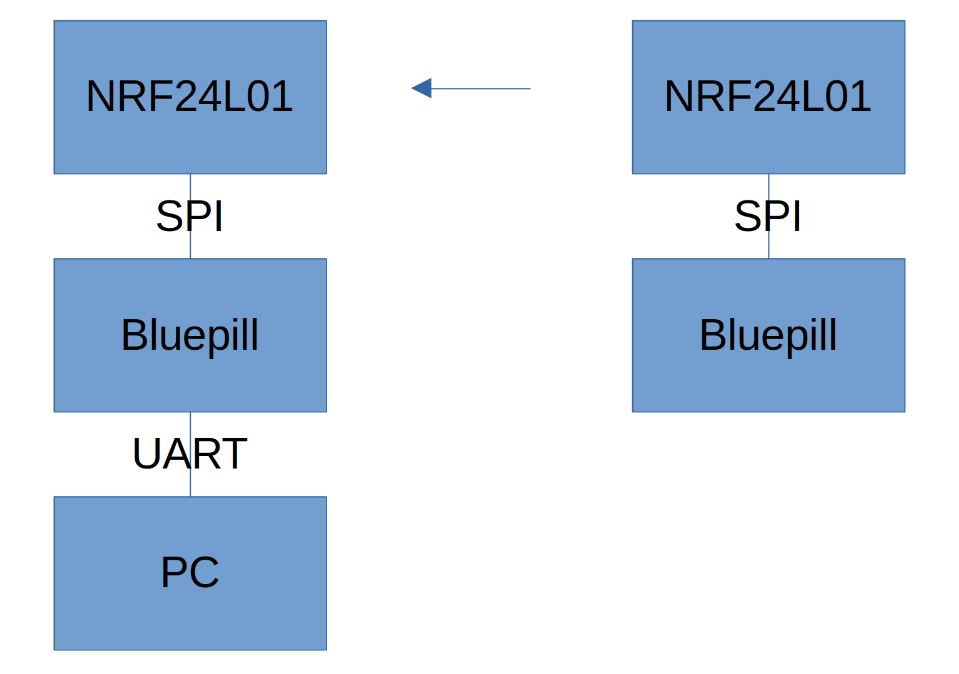
\includegraphics[width=0.5\textwidth]{Bloques.png}
    \caption{Diagrama en bloques del sistema propuesto.}
    \label{fig:SPI_write}
\end{figure}

\section{Arquitectura del hardware}

El sistema se divide en dos unidades funcionales con las siguientes características:

\textbf{Nodo transmisor: }

\begin{itemize}
	\item \textbf{Unidad de Procesamiento:} Microcontrolador STM32F103C8T6 (Blue Pill).
	\item \textbf{Interfaz de Radio:} Módulo nRF24L01 conectado mediante bus SPI.
	\item \textbf{Sensores:} Entrada para sensor ultrasónico JSN-SR04T (impermeable) para medición de nivel/distancia.
\end{itemize}

\textbf{Nodo receptor}

\begin{itemize}
	\item \textbf{Unidad de Procesamiento:} Microcontrolador STM32F103C8T6 (Blue Pill).
	\item \textbf{Interfaz de Radio:} Módulo nRF24L01 (SPI).
	\item \textbf{Interfaz de Usuario/PC:} Comunicación via UART hacia una PC para la visualización de datos mediante un terminal serie o interfaz gráfica.
	\item \textbf{Indicadores luminosos y sonoros:} Implementación de un display de segmentos verticales para indicar nivel y buzzer de alarma sonora.
\end{itemize}

\section{Especificaciones de Software y Protocolos}

Para la implementación de la lógica de control se utilizarán las siguientes herramientas y protocolos:

\begin{itemize}
	\item \textbf{Capa de Transporte Inalámbrico: }Protocolo propietario de Nordic Semiconductor (Enhanced ShockBurst™), configurando:
	\begin{itemize}
		\item Verificación de errores mediante CRC.
		\item Reintento automático de paquetes (Auto-ACK).
	\end{itemize}
	\item \textbf{Firmware:} Desarrollado en C utilizando las librerías HAL de STMicroelectronics.
	\item \textbf{SPI:} Configurado en Modo 0.
	\item \textbf{UART:} Configurada a 115200 bps para la transmisión de tramas hacia la PC.
\end{itemize}


\end{document}